% Two maps of Congress: 02805 final project paper.
% Built for the PNAS Overleaf template ("PNAS Template for Research Reports"). To use it: open the template in
% Overleaf, upload sections/, figures/ and references.bib, and replace the template's main file with this one.
% The class file pnas-new.cls comes with the template; it is not in this repository. See README.md.
\documentclass[9pt,twocolumn,twoside]{pnas-new}
\templatetype{pnasresearcharticle}

\title{Two maps of Congress: the House is less divided in whom its members name than in whom they work with}

\author[a]{Anas Mir}
\author[a]{Martin M{\o}llenhus}
\author[a]{Diego A. Mijares}
\affil[a]{Technical University of Denmark, 02805 Social Graphs and Interactions}

\leadauthor{Mir}

\significancestatement{% Significance statement: 120 words maximum in PNAS. First draft, Diego with Claude, 22 Nov.
Congress is described as two camps, usually from votes or vocabulary. We ask a narrower question: whom do members
name, and is that more divided than whom they work with? Comparing two networks of the same members, we find that
members name colleagues across the aisle more often than they cosponsor with them, and that these names are mostly
credit, not attack. Much of this follows from how floor debate is organised, so it describes the House's
procedures as much as its members' intentions. The result shows that measured polarization depends on the record
chosen, and it offers a check that words such as ``bipartisan'' do not: a named partner can be compared with the
legislative record.
}

\authorcontributions{% Author contributions: specific, as the course asks. Draft from WORK_AND_DEADLINES.md; each author checks their line.
M.M. built the floor and working maps, the shared name matcher and the mention table, the rewired, debate and state
null models and the community analysis, made Figure 1 and wrote the Results on the two maps and the Methods on data
and networks. A.M. built the press-release collector, collected 55,023 releases, matched them to members and bills,
measured district lean for redrawn states, ran the close-up analysis and its checks, the home map and the analysis
of ``bipartisan'' releases, made Figure 3 and wrote the Results on the close-up and the Methods on press releases.
D.A.M. measured the matcher's precision, wrote the labelling rules, coded the 100 labelled mentions, built the text
classifier, compiled the literature, made Figure 2 and wrote the Results on what mentions mean. M.M. and A.M. second-coded
the labelled mentions. D.A.M. and M.M. wrote the Introduction and Discussion. All authors read and revised the
paper. Code and text were drafted with an AI assistant (Claude, Anthropic), as listed in AI\_METHODS.md.
}
\authordeclaration{The authors declare no competing interest.}
\correspondingauthor{}

\keywords{Congress $|$ polarization $|$ networks $|$ floor speech $|$ cosponsorship}

\begin{abstract}
% Abstract: 150 words maximum (course rule). First draft, Diego with Claude, 22 Nov. Revise after the read-through.
Members of the US House vote along party lines, but how divided is the House in whom its members name? We draw
the 119th House (2025 to 2026) twice on the same 450 members: a working map, where two members are joined when one
cosponsors the other's bill, and a floor map, where they are joined when one names the other in a floor speech. At
equal size, 38.7\% of floor ties cross the party line against 28.6\% of working ties. Both maps are more divided
than rewired networks, and debate procedure explains about two thirds of the floor map's division. Reading 100
mentions by hand shows that cross-party mentions are mostly thanks and credit (69\%) and rarely disagreement (7\%).
In press releases, members in exposed seats name the other party more often than members in safe seats. How
divided Congress looks depends on which record is read.

\end{abstract}

\dates{Hand-in 27 November 2026.}

\begin{document}

\maketitle
\thispagestyle{firststyle}
\ifthenelse{\boolean{shortarticle}}{\ifthenelse{\boolean{singlecolumn}}{\abscontentformatted}{\abscontent}}{}

% Introduction. First draft, Diego with Claude, 22 Nov, on the frozen numbers. Diego and Martin write the
% Introduction and Discussion together (DECISIONS G3): Martin to revise. Budget about 0.75 page.

\dropcap{T}he United States Congress is usually described as two camps, and most ways of measuring it agree.
Members of the two parties vote apart, and they have used increasingly different words since the early 1990s
\cite{gentzkow2019}. Networks built from who signs whose bills show the same split, with ties between the parties
growing rarer and more hostile over four decades \cite{neal2020}.

How deep the split looks depends, however, on which record is read. Between 1973 and 2004, bipartisan agreement
fell in roll-call votes while staying far more stable in cosponsorship, because party leaders chose which bills
reached a vote \cite{harbridge2015}. Across communication channels the parties are always distinguishable, but more
so in front of national audiences than local ones \cite{green2024}. Division is a property of the measurement as
well as of the institution.

Members also have reasons to manage how divided they appear. Voters with weak party attachments reward a
bipartisan image \cite{harbridge2011}, and what members say to constituents is a strategic presentation of their
work \cite{grimmer2013}. That presentation need not match the work: floor speeches that call a bill bipartisan
mostly concern bills with trivial support from the other party, and a member's bipartisan rhetoric is unrelated to
their bipartisan votes \cite{westwood2022}.

We compare two records of the same 450 members of the House in the 119th Congress (2025 to 2026). The first is the
cosponsorship network \cite{fowler2006}: two members are tied when one signs a bill the other sponsors. The second
is, to our knowledge, new: two members are tied when one names the other in a floor speech. Both are networks on
identical nodes, so the same measures of party division apply to each and both can be tested against the same
null models. A word such as ``bipartisan'' costs nothing to say. A name points at a specific colleague, and what is
said about that colleague can be read.

Whether naming is more or less partisan than working cannot be guessed in advance. Members might attack the other
side in public and cooperate quietly, or display the few cross-party partners they have. We find that the floor map
is less divided by party than the working map at equal size (38.7\% of ties cross the aisle, against 28.6\%), that
debate procedure accounts for much, but not all, of the floor map's own party division, and that cross-party mentions are mostly
acknowledgement rather than argument. At home, in press releases, members in exposed seats name the other party
more often than members in safe seats.

% Results. Part 1 is Martin's text, generated from Martin/results_part1.md by report/md2tex.py.
% Part 2 is Diego's (with Claude), from Diego/d2_labelling/RESULTS.md and Diego/d5_classifier/results.txt.
% Part 3 is Anas's (with Claude): sections/results_part3.tex, a copy of Anas/results_part3.tex (edit there and copy),
% followed by Martin's M6 paragraph. Full length on purpose for the 25 Nov read-through.

\section*{Results}

\subsection*{Two maps of the same House}
% Generated by report/md2tex.py from Martin/results_part1.md. Do not edit by hand.
\textbf{Two maps of the same House.} We built two networks on the same 450 Republicans and Democrats of the 119th House. In the \emph{working map}, two members are tied if one cosponsored a bill or joint resolution that the other sponsored (46,513 ties). In the \emph{floor map}, two members are tied if one named the other in a floor speech, leaving out yields of debate time (3,970 ties from 8,469 mentions; Methods).

\textbf{The floor map is less divided by party than the working map.} 38.7\% of floor ties cross the aisle (Fig.~1\emph{A} and \emph{C}). The floor map is about twelve times sparser, so we compare it with working ties drawn at random at the same size: across 200 draws, 28.6\% of working ties cross the aisle (range 26.8\% to 30.6\%), and no draw comes within eight points of the floor map (Fig.~1\emph{B} and \emph{C}). Party modularity agrees: 0.112 for the floor map against 0.211 (0.193 to 0.230) for the draws (Fig.~1\emph{D}). Leaving out yields does not create the gap: with yields kept, the floor map is at 35.2\% against 28.7\%. Members' strongest working partnerships are far more partisan still: of the 3,970 pairs who share the most bills, 12.8\% cross the aisle.

\textbf{Both maps are more divided than chance, and the floor map's division is partly procedure.} If ties were rewired at random with every member keeping their number of ties, about half would cross the aisle and modularity would be near zero in both maps (Fig.~1\emph{C} and \emph{D}). Floor debate has a structure of its own: each debate has a cast, often with a manager from each party. Shuffling who is named only within each debate leaves a modularity of 0.074 (0.065 to 0.082 over 200 shuffles) against 0.112 observed. The debates thus account for about two thirds of the floor map's party division; the rest, members naming their own side beyond what the debate forces, exceeds every shuffle. State delegations account for almost none of it: keeping each member's number of ties within their own state gives a modularity of 0.001 (at most 0.023 over 200 draws).

\textbf{Communities follow party on one map and committees on the other.} On the working map, Louvain's communities are the two parties (normalised mutual information with party, NMI, 0.83). On the floor map they cut across party (NMI 0.03, against 0.29 for working draws of the same size): eight communities of 28 to 80 members, each holding both parties. In seven of them one House committee is 3.0 to 7.9 times as common as in the House as a whole, among them Appropriations (82\% of the community's members), Ways and Means (79\%) and Energy and Commerce (67\%); the eighth gathers the party leaders. 44\% of floor ties join two members of the same committee, against 17.1\% when ties are rewired at random, and so do 50\% of cross-party floor ties. In the working map the share barely exceeds chance (22\% against 18.7\%).

\textbf{In short,} members name colleagues of the other party on the floor more often than they cosponsor with them, and much of that naming runs between members of the same committee. Part 2 reads what these mentions say.


\begin{figure*}[t]
\centering
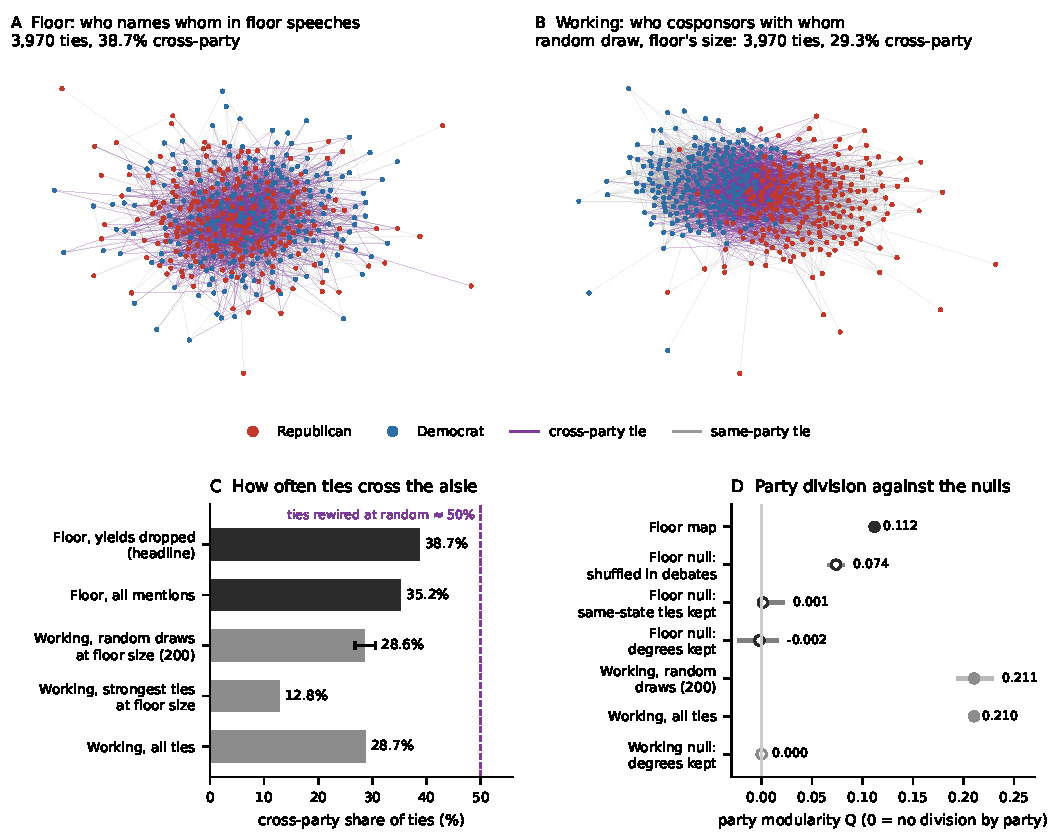
\includegraphics[width=17.8cm]{figures/figure1.pdf}
% Generated by report/md2tex.py from Martin/results_part1.md. Do not edit by hand.
\caption{The House as two networks, January 2025 to November 2026. (\emph{A}) Floor map: members tied when one names the other in a floor speech, yields of debate time left out. (\emph{B}) Working map: one random draw of sponsor–cosponsor ties, thinned to the floor map's 3,970 ties. Nodes are members (red Republican, blue Democrat); purple ties cross the aisle. Positions come from a spring layout and carry no meaning. (\emph{C}) Share of ties that cross the aisle; the bar for the random draws shows the range over 200 draws, and the dashed line the level expected if ties were rewired at random. (\emph{D}) Party modularity of each map (filled) against its nulls (open; lines show the range over the draws): shuffling who is named within each debate, keeping each member's same-state ties, and keeping each member's number of ties.}

\label{fig:maps}
\end{figure*}

\subsection*{What a cross-party mention means}

Naming a colleague is not working with them, and a member can name the other side to attack it. To find out what
the floor map's cross-party ties are, we read 100 floor mentions drawn at random, 75 between parties and 25 within
a party, and coded what the speaker was doing towards the named member (Methods). Of the cross-party mentions, 69\%
(95\% interval 58\% to 79\%) were agreeing: thanks to a bill's co-lead or to a committee's chair, praise for joint
work, support for the member's bill. 23\% (15\% to 33\%) were neutral references, such as the member who
introduced a bill or whose district a constituent lives in. Only 7\% (3\% to 15\%) disagreed with the named member
(Fig.~\ref{fig:labels}). None was procedure: handing over debate time stays within a party (12\% of same-party
mentions). Two coders agreed on 82\% of the mentions (Cohen's $\kappa = 0.64$).

A text classifier trained on these labels could not carry them to all 9,909 floor mentions. Predicting each label
from a model trained on the other 99, it was right 73\% of the time, against 72\% for always answering
``agreeing'', and it found none of the five disagreements. We therefore report the hand-labelled shares only.

The floor map's cross-party ties are thus mostly acknowledgement, not argument. Members name the other side to
credit it far more often than to oppose it. The labels check that each name is the right member, but not which
members were missed: in 30 turns read in full, the matcher found 12 of the 13 members a reader found.

\begin{figure}[t]
\centering
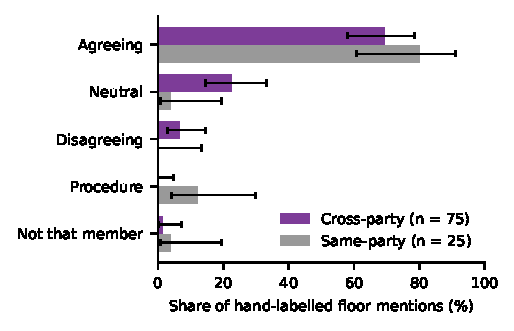
\includegraphics[width=8.7cm]{figures/figure2.pdf}
\caption{What floor mentions do. Share of 100 hand-labelled mentions in each code, for mentions between parties
(purple, $n = 75$) and within a party (grey, $n = 25$). Lines show 95\% Wilson intervals. Codes as in Methods; a
mention was coded ``not that member'' when the matched name referred to someone else.}
\label{fig:labels}
\end{figure}

\subsection*{Close-up: whom members name at home}
% Results, part 3: whom members name at home. Anas (with Claude), rewritten Mon 23 Nov 2026 (evening) at full length,
% after checks T and I (a4/CHECKS_PLAN_23NOV.md, designs fixed before running). One aim, with the detours kept:
% where the text count, the network, A5 and the checks disagree, the disagreement is stated and discussed.
% NOT cut to the word budget on purpose: every layer is here for the group's read-through (Wed 25 Nov), which decides
% what stays. Paragraphs marked [G17] are the optional extensions (home map, A5) the group still has to accept.
%
% Sources (all on the 22 Nov rerun; frozen inputs bc1c2344):
%   P1-P2  a4/out/results.csv, member_shares.csv, leave_one_state_out.csv; Figure 3. Range 7.9-10.1% = Figure 3A's
%          5-point bands beyond 5 points of own-party lean (bands with >= 5 members).
%   P3     check T: a4/check_tone/scored.csv (a4/README.md, "Check T").
%   P4     check I: a4/out/ideology_check.csv (a4/README.md, "Check I"); bands from members.csv nominate_dim1.
%   P5     home map: a4/out/home_measures_centrality.csv, home_measures_null.csv, home_ties.csv, alpha_centrality.csv
%          (a4/NETWORK_METHODS.md 3a, 3d).
%   P6     A5: a5/out/results.csv, a5/check/scored.csv, a5/mirror/scored.csv (a5/README.md).
% Martin's M6 paragraph (% Generated by report/md2tex.py from Martin/results_part1.md. Do not edit by hand.
\textbf{Do members show their cross-party bills at home?} Of the bills a member sponsored, those with an original cosponsor from the other party were cited in that member's press releases more often than their other bills (52.7\% against 45.1\%; 388 members, 10,125 bills). Shuffling, within each member, which bills count as cross-party gives a null in which the observed count is 1.08 times the expected (p < 0.001), in both parties. Most of the gap, however, separates co-led bills from solo bills: against bills co-led only by the member's own party, cross-party bills are cited 3.5 points more often (52.6\% against 49.1\%, p = 0.02). As original cosponsors, members cite the cross-party bills they join about three times as often as same-party ones (8.6\% against 2.9\%). We cannot rule out that bipartisan bills are cited more because they more often pass.
) follows this file in results.tex.
% To use: replace the placeholder under "Close-up" in report/sections/results.tex with % Results, part 3: whom members name at home. Anas (with Claude), rewritten Mon 23 Nov 2026 (evening) at full length,
% after checks T and I (a4/CHECKS_PLAN_23NOV.md, designs fixed before running). One aim, with the detours kept:
% where the text count, the network, A5 and the checks disagree, the disagreement is stated and discussed.
% NOT cut to the word budget on purpose: every layer is here for the group's read-through (Wed 25 Nov), which decides
% what stays. Paragraphs marked [G17] are the optional extensions (home map, A5) the group still has to accept.
%
% Sources (all on the 22 Nov rerun; frozen inputs bc1c2344):
%   P1-P2  a4/out/results.csv, member_shares.csv, leave_one_state_out.csv; Figure 3. Range 7.9-10.1% = Figure 3A's
%          5-point bands beyond 5 points of own-party lean (bands with >= 5 members).
%   P3     check T: a4/check_tone/scored.csv (a4/README.md, "Check T").
%   P4     check I: a4/out/ideology_check.csv (a4/README.md, "Check I"); bands from members.csv nominate_dim1.
%   P5     home map: a4/out/home_measures_centrality.csv, home_measures_null.csv, home_ties.csv, alpha_centrality.csv
%          (a4/NETWORK_METHODS.md 3a, 3d).
%   P6     A5: a5/out/results.csv, a5/check/scored.csv, a5/mirror/scored.csv (a5/README.md).
% Martin's M6 paragraph (\input{sections/from_martin_m6}) follows this file in results.tex.
% To use: replace the placeholder under "Close-up" in report/sections/results.tex with \input{sections/results_part3}.
% About 930 words after the humanizer pass (23 Nov); every number of the earlier version kept. Cuts: Wednesday.

\textbf{Members in exposed seats name the other party more often at home, in both parties.} We asked whom members name in their own press releases, and whether members whose seat is at risk name the other party more. For each of the 406 members with at least ten releases (53,664 releases, 3 January 2025 to 20 November 2026), we measured the share of releases naming a House member of the other party who is neither a party leader nor a co-lead of a bill the release cites. A seat is exposed when the district the member served leans toward their own party by five points or less (Cook PVI 2025). Exposed Republicans named Democrats in 13.3\% of their releases, against 9.2\% for safe Republicans; exposed Democrats named Republicans in 11.6\%, against 9.0\% (permutation $p = 0.004$ for each; Fig.~\ref{fig:home}). The two gaps differ by 1.5 points ($p = 0.36$), too little to tell whether being in the president's party matters.

\textbf{The difference sits in the closest seats.} Members whose district is even or leans to the other party named the other party most (Republicans 19.2\%, $n = 8$; Democrats 14.2\%, $n = 10$). Beyond five points of lean the share is nearly flat, between 7.9\% and 10.1\% (Fig.~\ref{fig:home}\emph{A}). Every check fixed before the analysis gives a positive gap in both parties with $p < 0.05$: other cut-offs, the 2024 presidential margin instead of Cook, leaving out the 21 members whose label changes or is unknown under the 2026 maps, leaving out releases about redistricting or caucuses, and the floor's matcher without the press additions (Fig.~\ref{fig:home}\emph{B}). The gaps keep their sign when any one state is left out, and widen to 7.0 and 6.3 points when co-leads count too.

\textbf{Most of the names are partners.} A count says nothing about tone, and an exposed member could name the other side to attack it. Three blind AI readers, who did not see the seat, coded 60 counted names, 15 for each party and seat: 46 named a partner or praised the member (77\%), 9 were neutral mentions such as a committee chair addressed in a letter, 4 were wrong matches, and one criticised (a safe Republican on a Democrat's remarks). Exposed and safe seats did not differ in criticism. At home, as on the floor, cross-party names are mostly acknowledgement.

\textbf{Exposed members are also their party's moderates, and the two cannot be separated.} Of the 37 exposed Republicans, 22 are in their party's most moderate fifth by DW-NOMINATE, as are 27 of the 54 exposed Democrats; the most extreme fifths hold 3 and 2. Shuffling the exposed label only among members of the same party and ideology band gives the gap ideology alone would produce: 2.9 of the 4.1 Republican points and 2.4 of the 2.6 Democratic points. The remainder (1.1 and 0.2 points) cannot be told from chance ($p = 0.39$ and $0.76$), so our data cannot say whether the seat or the member's ideology drives the naming. The test is strict: DW-NOMINATE comes from roll-call votes, and members may vote moderately because their seat is close, so holding it fixed can remove part of a real seat effect. More of the Republican gap survives, a party difference that returns in the network.

% [G17] Home map (network extension): keep or cut on Wednesday. Its comparisons inherit the ideology caveat (not tested).
% If kept: the 'majority's control of committees' clause is untested. Possible test, decided 23 Nov to wait for Wednesday:
% sort counted cross-party names by route (same committee / bill release / other), exposed vs safe by party
% (Martin/m5_committees, a3 bill links), design written first, labelled exploratory. About 1.5 h. See a4/README.md.
\textbf{The network sees the two parties differently.} Tying two members when one names the other gives a home map of the same 406 members. In both parties exposed members are its hubs: they are 22\% of members but send 35\% and receive 34\% of its cross-party ties, and are tied to 1.9 times (Republicans) and 1.5 times (Democrats) as many members of the other party as safe members are (Holm-corrected $p = 0.001$ for each). On the backbone, which keeps each member's strongest ties, the parties split. Exposed Republicans have 1.5 times the backbone ties of safe Republicans (Holm $p = 0.013$), with borderline higher betweenness and closeness (Holm $p = 0.059$ and $0.055$): they bridge by volume. Exposed Democrats have as many backbone ties and as central a position as safe Democrats, but sit on more shortest paths than their ties predict (Holm $p = 0.08$ at our backbone level, below 0.05 at every looser one): they bridge by position. So one gap in the text hides two roles in the network. We did not test why; one possibility is that the majority's control of committees and the floor agenda gives exposed Republicans more occasions to name Democrats. Exposed members tie to each other only slightly more than their activity predicts (10.7\% of cross-party ties join two exposed members, against 10.2\% when ties are rewired with every member's number of ties kept; $p = 0.015$).

% [G17] A5 ("bipartisan"): keep or cut on Wednesday. Not tested against ideology.
\textbf{The word ``bipartisan'' mostly comes with a partner, and here the parties swap.} A quarter of the releases (13,744) call something bipartisan. In 64\% of them a House member of the other party is named or co-leads a cited bill, against 9\% of other releases (means over 370 members). Three blind AI readers checked 30 releases of each kind: of those naming a member of the other party, 28 named a partner and none an opponent; of those naming none, 29 named no partner from the other party and one named a senator, whom our matcher does not count. By seat, the difference runs the other way from the backbone: exposed Democrats back the word with a partner more often than safe Democrats (63.0\% against 56.7\%, $p = 0.012$), while exposed and safe Republicans do not differ (72.1\% against 69.1\%, $p = 0.40$) and both exceed Democrats (not tested).
.
% About 930 words after the humanizer pass (23 Nov); every number of the earlier version kept. Cuts: Wednesday.

\textbf{Members in exposed seats name the other party more often at home, in both parties.} We asked whom members name in their own press releases, and whether members whose seat is at risk name the other party more. For each of the 406 members with at least ten releases (53,664 releases, 3 January 2025 to 20 November 2026), we measured the share of releases naming a House member of the other party who is neither a party leader nor a co-lead of a bill the release cites. A seat is exposed when the district the member served leans toward their own party by five points or less (Cook PVI 2025). Exposed Republicans named Democrats in 13.3\% of their releases, against 9.2\% for safe Republicans; exposed Democrats named Republicans in 11.6\%, against 9.0\% (permutation $p = 0.004$ for each; Fig.~\ref{fig:home}). The two gaps differ by 1.5 points ($p = 0.36$), too little to tell whether being in the president's party matters.

\textbf{The difference sits in the closest seats.} Members whose district is even or leans to the other party named the other party most (Republicans 19.2\%, $n = 8$; Democrats 14.2\%, $n = 10$). Beyond five points of lean the share is nearly flat, between 7.9\% and 10.1\% (Fig.~\ref{fig:home}\emph{A}). Every check fixed before the analysis gives a positive gap in both parties with $p < 0.05$: other cut-offs, the 2024 presidential margin instead of Cook, leaving out the 21 members whose label changes or is unknown under the 2026 maps, leaving out releases about redistricting or caucuses, and the floor's matcher without the press additions (Fig.~\ref{fig:home}\emph{B}). The gaps keep their sign when any one state is left out, and widen to 7.0 and 6.3 points when co-leads count too.

\textbf{Most of the names are partners.} A count says nothing about tone, and an exposed member could name the other side to attack it. Three blind AI readers, who did not see the seat, coded 60 counted names, 15 for each party and seat: 46 named a partner or praised the member (77\%), 9 were neutral mentions such as a committee chair addressed in a letter, 4 were wrong matches, and one criticised (a safe Republican on a Democrat's remarks). Exposed and safe seats did not differ in criticism. At home, as on the floor, cross-party names are mostly acknowledgement.

\textbf{Exposed members are also their party's moderates, and the two cannot be separated.} Of the 37 exposed Republicans, 22 are in their party's most moderate fifth by DW-NOMINATE, as are 27 of the 54 exposed Democrats; the most extreme fifths hold 3 and 2. Shuffling the exposed label only among members of the same party and ideology band gives the gap ideology alone would produce: 2.9 of the 4.1 Republican points and 2.4 of the 2.6 Democratic points. The remainder (1.1 and 0.2 points) cannot be told from chance ($p = 0.39$ and $0.76$), so our data cannot say whether the seat or the member's ideology drives the naming. The test is strict: DW-NOMINATE comes from roll-call votes, and members may vote moderately because their seat is close, so holding it fixed can remove part of a real seat effect. More of the Republican gap survives, a party difference that returns in the network.

% [G17] Home map (network extension): keep or cut on Wednesday. Its comparisons inherit the ideology caveat (not tested).
% If kept: the 'majority's control of committees' clause is untested. Possible test, decided 23 Nov to wait for Wednesday:
% sort counted cross-party names by route (same committee / bill release / other), exposed vs safe by party
% (Martin/m5_committees, a3 bill links), design written first, labelled exploratory. About 1.5 h. See a4/README.md.
\textbf{The network sees the two parties differently.} Tying two members when one names the other gives a home map of the same 406 members. In both parties exposed members are its hubs: they are 22\% of members but send 35\% and receive 34\% of its cross-party ties, and are tied to 1.9 times (Republicans) and 1.5 times (Democrats) as many members of the other party as safe members are (Holm-corrected $p = 0.001$ for each). On the backbone, which keeps each member's strongest ties, the parties split. Exposed Republicans have 1.5 times the backbone ties of safe Republicans (Holm $p = 0.013$), with borderline higher betweenness and closeness (Holm $p = 0.059$ and $0.055$): they bridge by volume. Exposed Democrats have as many backbone ties and as central a position as safe Democrats, but sit on more shortest paths than their ties predict (Holm $p = 0.08$ at our backbone level, below 0.05 at every looser one): they bridge by position. So one gap in the text hides two roles in the network. We did not test why; one possibility is that the majority's control of committees and the floor agenda gives exposed Republicans more occasions to name Democrats. Exposed members tie to each other only slightly more than their activity predicts (10.7\% of cross-party ties join two exposed members, against 10.2\% when ties are rewired with every member's number of ties kept; $p = 0.015$).

% [G17] A5 ("bipartisan"): keep or cut on Wednesday. Not tested against ideology.
\textbf{The word ``bipartisan'' mostly comes with a partner, and here the parties swap.} A quarter of the releases (13,744) call something bipartisan. In 64\% of them a House member of the other party is named or co-leads a cited bill, against 9\% of other releases (means over 370 members). Three blind AI readers checked 30 releases of each kind: of those naming a member of the other party, 28 named a partner and none an opponent; of those naming none, 29 named no partner from the other party and one named a senator, whom our matcher does not count. By seat, the difference runs the other way from the backbone: exposed Democrats back the word with a partner more often than safe Democrats (63.0\% against 56.7\%, $p = 0.012$), while exposed and safe Republicans do not differ (72.1\% against 69.1\%, $p = 0.40$) and both exceed Democrats (not tested).


% Generated by report/md2tex.py from Martin/results_part1.md. Do not edit by hand.
\textbf{Do members show their cross-party bills at home?} Of the bills a member sponsored, those with an original cosponsor from the other party were cited in that member's press releases more often than their other bills (52.7\% against 45.1\%; 388 members, 10,125 bills). Shuffling, within each member, which bills count as cross-party gives a null in which the observed count is 1.08 times the expected (p < 0.001), in both parties. Most of the gap, however, separates co-led bills from solo bills: against bills co-led only by the member's own party, cross-party bills are cited 3.5 points more often (52.6\% against 49.1\%, p = 0.02). As original cosponsors, members cite the cross-party bills they join about three times as often as same-party ones (8.6\% against 2.9\%). We cannot rule out that bipartisan bills are cited more because they more often pass.


\begin{figure}[t]
\centering
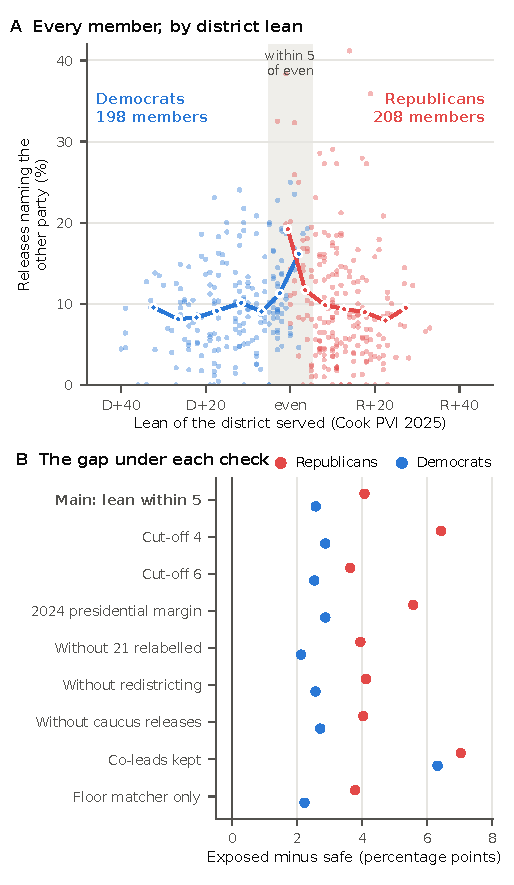
\includegraphics[width=8.7cm]{figures/figure3.pdf}
\caption{\textbf{Members in exposed seats name the other party more often in their press releases.} (\emph{A}) Each dot is one of 406 House members (198 Democrats, 208 Republicans; 53,664 releases, 3 January 2025 to 20 November 2026): the share of their releases that name a House member of the other party who is neither a party leader nor a co-lead of a bill the release cites, against the lean of the district they served (Cook PVI 2025). Lines join the mean share in 5-point bands of lean (bands with at least five members). Shading marks districts within five points of even; a member counts as exposed when the district leans toward their own party by five points or less, which includes seats leaning to the other party. (\emph{B}) Exposed minus safe mean share, by party, for the main definition (top) and for each check fixed before the analysis: other cut-offs, the 2024 presidential margin as lean, leaving out the 21 members relabelled or unplaced under the 2026 maps, leaving out releases about redistricting or caucuses, counting co-leads, and the floor's matcher without the press additions. Every gap is positive with $p < 0.05$ (labels shuffled within party, 10,000 shuffles).}
\label{fig:home}
\end{figure}

% Discussion. First draft, Diego with Claude, 22 Nov, on the frozen numbers. Martin to revise (DECISIONS G3).
% Budget about 0.75 page, limitations included.

\section*{Discussion}

Drawn from the same members over the same two years, the House looks less divided in whom its members name on the
floor than in whom they work with. The difference holds when both maps have the same number of ties, when yields
of debate time are left out, and against a null model that keeps who took part in each debate. Hand-labelled
mentions say what the cross-party ties are: mostly thanks and credit, rarely argument. The floor is where
cross-party work is acknowledged, typically by the managers of a bill and the leaders of its committee.

The result does not show that members cooperate more than cosponsorship suggests. A mention is a reference, made
in a setting where House procedure brings members of both parties into the same debates; that procedure accounts
for about two thirds of the floor map's party division, and the communities of the floor map follow committees,
not parties. Part of what we measure is therefore the committee system at work in public. The comparison also
depends on how the dense working map is thinned: against random ties of the same number the gap is ten points,
against members' strongest partnerships (12.8\% cross-party) it is much wider.

Several limits are our own findings. The name matcher was right in 98 of 100 hand-labelled mentions and found 12
of 13 names in 30 turns read in full, so recall rests on few names. Wrong matches are not neutral: a constituent or a
namesake mistaken for a member belongs to the other party about half the time, and on an earlier version of the
matcher five of seven errors joined members of different parties. Errors of this kind push the floor map towards
looking less divided; at 98\% precision the effect on the headline is small, but it runs in the direction of our
finding. One hundred labels give wide intervals and too few
disagreements for a text classifier to learn from: ours did not beat always answering ``agreeing''. Party was hidden on the
coding sheets, but coders often know a member's party, so the coding was not blind in practice. [S2: speaker attribution, result to
add.]

Where Westwood found that the word ``bipartisan'' is detached from votes \cite{westwood2022}, the names members use
across the aisle on the floor are mostly credit for specific bills and committee work. We did not test, pair by
pair, whether each named colleague is also a cosponsorship partner; that is the natural next check. At home the picture is a choice: members in exposed seats show
the other party more often than members in safe seats, in both parties. One Congress and one chamber cannot say
whether these patterns are stable. The same two maps can be drawn for any Congress since the Record went online.


\matmethods{% Methods. Budget about 1.25 pages for all of it; cut at the Wednesday read-through.
% Data, name matching, yields, maps, nulls, communities: Martin, generated from Martin/methods_networks.md.
% Labelling and classifier: Diego with Claude. Press releases: Anas (to write, from Anas/methods_drafts.md).

% Generated by report/md2tex.py from Martin/methods_networks.md. Do not edit by hand.
\textbf{Data.} Members are the 450 Republicans and Democrats who served in the 119th House, identified by Bioguide ID (Voteview, with unitedstates/congress-legislators for names). Floor speech comes from the Congressional Record on govinfo.gov, 6 January 2025 to 9 November 2026, split into speaker turns; we keep the 17,824 House-floor turns of at least 50 words spoken by a member. Bills and cosponsorships come from govinfo's BILLSTATUS bulk data for the same Congress. Whether each turn is attributed to the right speaker was checked by hand on 60 turns drawn at random: all 60 were assigned to the member the Record names as speaker (95\% Wilson interval 94\% to 100\%).

\textbf{Finding names.} A rule-based matcher finds each member named in a turn: a House title followed by a surname (``Mr. Cole'', ``Chairman Cole'', ``Speaker Johnson''), names in lists after a plural title (``Representatives Lawler, Golden, and Fitzpatrick''), and full names without a title (``my friend, Chip Roy''). Shared surnames are settled by first name (official or nickname) and then by a state name within 80 characters; otherwise the name is dropped. Possessives and middle initials are read through; names after ``State'', ``Senator'', ``Governor'' and similar titles are skipped. A member naming themselves is not counted. On 100 hand-labelled mentions, 98 named the right member (precision; Diego's sample, drawn before lists and untitled names were added; those two forms were checked separately, 20 of 20 and 30 of 30 right); in 30 randomly drawn turns, the matcher found 12 of the 13 members a reader found (recall, 92\%). The one miss was an unresolved shared surname.

\textbf{Yields.} When a floor manager hands debate time to a member (``I yield 2 minutes to the gentleman from Texas''), the name is procedure, not a choice to name someone. We flag a mention as a yield when ``yield'' (not ``yield back'') precedes the name in the same sentence, or ``for yielding'' follows it, and leave yields out of the headline floor map. On 30 held-out mentions where this rule and a simpler 60-character window disagreed, all 15 mentions only our rule flagged were yields, and 14 of the 15 only the window flagged were not.

\textbf{The two maps.} Both maps are undirected and unweighted, on the same members. Floor: two members are tied if either named the other at least once (3,970 ties from 8,469 mentions without yields). Working: two members are tied if one cosponsored a bill or joint resolution that the other sponsored, withdrawn cosponsorships removed (46,513 ties). Because the working map is about twelve times denser, we compare the floor map with 200 random draws of working ties of the same size, and separately with the 3,970 strongest working ties (pairs sharing the most bills).

\textbf{Division and nulls.} We measure division by party as the share of ties that cross the aisle and as modularity Q of the party split. Each map is compared with three nulls: (i) degree-preserving rewiring (double-edge swaps, five per tie, 200 rewirings; 20 for the full working map), which keeps how many ties each member has; (ii) for the floor map, a shuffle of who is named within each debate (one Congressional Record item; five swaps per mention, 200 shuffles), which keeps who speaks and who is named in each debate; and (iii) a rewiring that also keeps each member's number of ties within their own state (200 draws). Seed 2805 throughout.

\textbf{Communities.} We find communities with the Louvain method (resolution 1, 50 random starts, keeping the partition with the highest modularity) and compare them with party, and between maps, by normalised mutual information. To ask what the floor communities are, we use current House committee assignments (unitedstates/congress-legislators, downloaded 22 November 2026) and count the floor ties that join two members of the same full committee, against the same degree-preserving rewiring.


\textbf{Labelling what a mention does.} We drew 100 floor mentions at random with a fixed seed, 75 between members
of different parties and 25 within a party, from the mentions found on 18 November (before lists and untitled
names were added to the matcher). Coders saw the speaker, the named member, the date and three sentences of
context, but not the parties. Each mention got one of five codes for what the speaker did towards the named member:
procedure (handing over or thanking for debate time), agreeing (thanks, praise, partnership, support for the
member's bill), disagreeing (rebuttal, criticism, blame, a demand to change course), neutral (a reference that takes
no side), or not that member (a wrong match, or Record text the speaker did not say). The rules for mixed cases were
fixed before coding; where two codes fitted, the first in the order not that member, procedure, disagreeing,
agreeing, neutral was used. One author coded all 100 mentions. A second author coded 25 of them each (50 in all),
and an AI assistant (Claude) coded the other 50 following the same written rules, without seeing any human code.
Agreement between the human coders was 82\% (Cohen's $\kappa = 0.64$; 0.59 and 0.69 for the two pairs), and between
the first coder and the AI coder 88\% ($\kappa = 0.72$). Three further independent runs of the AI coder on all 100
mentions agreed with each other on 99 or 100 and with the first coder on 81\% to 82\% ($\kappa$ 0.56 to 0.58); being
the same model, they show that its coding is stable, not that it is right. Shares are reported from the first
coder's codes with 95\% Wilson intervals. The first coder changed two codes to ``not that member'' after the AI
coders flagged them; both were clear matcher errors (a port authority's director and a member's late husband).

\textbf{Classifier.} To carry the labels to all floor mentions we trained a logistic-regression classifier (classes
weighted by inverse frequency, $C = 1$, not tuned) on TF-IDF features of each mention's context: words and word
pairs occurring in at least two mentions, with the named member's surname replaced by a placeholder. We tested it
with leave-one-out cross-validation on the 100 labelled mentions and compared it with always predicting the most
common code. It did not beat that baseline (73\% against 72\% accuracy, macro F1 0.26, no disagreement found), so
its predictions are not used as measurements.

\textbf{Press releases.} [Anas: collection (55,023 releases from 412 members, members' house.gov sites, snapshot
20 November 2026), matching releases to bills by number and marking co-leads (A3), district lean of the seat
served (Cook PVI 2025, with the 2024 presidential margin as a check), the definition of an exposed seat, and the
permutation test. Sources: \texttt{Anas/methods\_drafts.md}, \texttt{Anas/a4/README.md}, \texttt{Anas/a3/README.md}.
Martin's M6 null: own bills are sponsored H.R. and H.J.Res.; cross-party means an original cosponsor of the other
party; the cross-party label is shuffled within each member, 10,000 shuffles.]

\textbf{AI use.} Code, data checks and drafts of the text were written with an AI assistant (Claude, Anthropic).
Every place a model touched a result, and how it was checked, is listed in \texttt{AI\_METHODS.md} in the project
repository.

\textbf{Data and code.} [repository link] \cite{fowler2006,newman2006,maslov2002,serrano2009,blondel2008,danon2005,landis1977}
}

\showmatmethods{}

\bibliography{references}

\end{document}
